\documentclass[12pt,a4paper]{article}
\usepackage[utf8]{vietnam}
\usepackage{amsmath,amssymb}
\usepackage{tabularx}
\usepackage{tikz}
\usetikzlibrary{calc,angles,quotes,arrows.meta,patterns}
\usepackage{xcolor}
\usepackage{enumitem}
\usepackage{fancyhdr}
\usepackage{graphicx}
\usepackage[top=0.9cm, bottom=0.9cm, left=1.2cm, right=1.2cm]{geometry}
\usepackage[loigiai]{ex_test}
\SAOPTN{widthSA=3.2,heightSA=0.62}

\setlength{\headheight}{15pt}
\setlength{\parskip}{0pt}

\pagestyle{fancy}
\fancyhf{}
\rhead{\textit{Môn Toán 8 -- Hướng dẫn giải Đề số 09}}
\lhead{\textit{Bộ đề ôn tập Giữa học kì I}}
\cfoot{\thepage}

\begin{document}

\begin{center}
  \textbf{\Large HƯỚNG DẪN GIẢI CHI TIẾT VÀ BẢNG ĐÁP ÁN}\\
  \textbf{\large ĐỀ ÔN TẬP GIỮA HỌC KỲ I -- ĐỀ SỐ 09}\\
  \textit{Môn: Toán 8 -- Năm học 2026 -- 2027}
\end{center}
\vspace{2mm}

% --- BẢNG ĐÁP ÁN TRẮC NGHIỆM TÓM TẮT ---
\noindent\textbf{\large A. BẢNG ĐÁP ÁN TRẮC NGHIỆM TỔNG HỢP}
\vspace{1mm}

\noindent\textbf{1. Phần I (Mỗi câu trả lời đúng được 0,25 điểm):}
\begin{center}
\begin{tabular}{|c|c|c|c|c|c|c|c|c|c|c|c|c|}
\hline
\textbf{Câu} & \textbf{1} & \textbf{2} & \textbf{3} & \textbf{4} & \textbf{5} & \textbf{6} & \textbf{7} & \textbf{8} & \textbf{9} & \textbf{10} & \textbf{11} & \textbf{12} \\
\hline
\textbf{Đ/A} & \textbf{B} & \textbf{C} & \textbf{A} & \textbf{D} & \textbf{B} & \textbf{B} & \textbf{A} & \textbf{C} & \textbf{C} & \textbf{A} & \textbf{B} & \textbf{B} \\
\hline
\end{tabular}
\end{center}
\vspace{0.5mm}

\noindent\textbf{2. Phần II (Đúng 1 ý: 0,1đ; 2 ý: 0,25đ; 3 ý: 0,5đ; 4 ý: 1,0đ):}
\begin{center}
\begin{tabular}{|c|c|c|c|c||c|c|c|c|c|}
\hline
\textbf{Câu} & \textbf{a)} & \textbf{b)} & \textbf{c)} & \textbf{d)} & \textbf{Câu} & \textbf{a)} & \textbf{b)} & \textbf{c)} & \textbf{d)} \\
\hline
\textbf{Câu 1} & \textbf{Đ} & \textbf{S} & \textbf{Đ} & \textbf{Đ} & \textbf{Câu 2} & \textbf{Đ} & \textbf{Đ} & \textbf{S} & \textbf{Đ} \\
\hline
\end{tabular}
\end{center}
\vspace{0.5mm}

\noindent\textbf{3. Phần III (Mỗi câu trả lời đúng được 1,0 điểm):}
\begin{center}
\begin{tabular}{|c|c|c|}
\hline
\textbf{Câu} & \textbf{Câu 1} & \textbf{Câu 2} \\
\hline
\textbf{Đáp án} & $\mathbf{x = -4 \text{ hoặc } x = 6}$ & $\mathbf{5\text{ cm}}$ \\
\hline
\end{tabular}
\end{center}
\vspace{1.5mm}

% --- B. LỜI GIẢI CHI TIẾT ---
\noindent\textbf{\large B. LỜI GIẢI CHI TIẾT CÁC CÂU HỎI}
\vspace{1mm}
\begin{ex}
Trong các biểu thức sau, biểu thức nào là đơn thức?
\choice
{$\dfrac{1}{x} + y$}
{\True $2xy^2$}
{$(2 - x)y^2$}
{$\sqrt{x - y}$}
\loigiai{
Đơn thức là biểu thức đại số chỉ gồm một số, một biến, hoặc một tích giữa các số và các biến. Biểu thức $2xy^2$ là đơn thức.
}
\end{ex}

\begin{ex}
Tích của hai đơn thức $\dfrac{1}{2}xy^3$ và $(-8x^2yz^2)$ có phần hệ số là:
\choice
{$\dfrac{1}{2}$}
{$-8$}
{\True $-4$}
{$7$}
\loigiai{
Ta có: $\dfrac{1}{2}xy^3 \cdot (-8x^2yz^2) = -4x^3y^4z^2$. Phần hệ số là $-4$.
}
\end{ex}

\begin{ex}
Hình thang cân là hình thang có:
\choice
{\True Hai góc kề một đáy bằng nhau}
{Hai góc đối bằng nhau}
{Hai cạnh đối bằng nhau}
{Hai đường chéo vuông góc với nhau}
\loigiai{
Theo định nghĩa, hình thang cân là hình thang có hai góc kề một đáy bằng nhau.
}
\end{ex}

\begin{ex}
Kết quả khai triển biểu thức $(x - 2)(x - 2)$ là:
\choice
{$x^2 + 2x + 4$}
{$x^2 + 4x + 4$}
{$x^2 - 2x + 4$}
{\True $x^2 - 4x + 4$}
\loigiai{
Ta có: $(x - 2)(x - 2) = (x - 2)^2 = x^2 - 4x + 4$.
}
\end{ex}

\begin{ex}
Chọn câu sai trong các câu sau:
\choice
{Tứ giác có 3 góc tù, 1 góc nhọn}
{\True Tứ giác có 3 góc vuông, 1 góc nhọn}
{Tứ giác có nhiều nhất 2 góc tù, nhiều nhất 2 góc nhọn}
{Tứ giác có 3 góc nhọn, 1 góc tù}
\loigiai{
Tổng 4 góc trong tứ giác bằng $360^\circ$. Nếu có 3 góc vuông thì góc thứ tư phải bằng $360^\circ - 3 \cdot 90^\circ = 90^\circ$ (góc vuông), không thể là góc nhọn. Do đó B là câu sai.
}
\end{ex}

\begin{ex}
Tứ giác có hai cạnh đối song song là:
\choice
{Hình thang cân}
{\True Hình thang}
{Hình bình hành}
{Hình chữ nhật}
\loigiai{
Theo định nghĩa, hình thang là tứ giác có hai cạnh đối song song.
}
\end{ex}

\begin{ex}
Giá trị của biểu thức $A = x^3y + 7x^2y + 9$ tại $x = -1, y = 2$ là:
\choice
{\True $21$}
{$25$}
{$-7$}
{$-3$}
\loigiai{
Thay $x = -1, y = 2$ vào biểu thức $A$: $A = (-1)^3 \cdot 2 + 7(-1)^2 \cdot 2 + 9 = -2 + 14 + 9 = 21$.
}
\end{ex}

\begin{ex}
Chọn đẳng thức sai trong các đẳng thức sau đây:
\choice
{$(a + b)^3 = a^3 + 3a^2b + 3ab^2 + b^3$}
{$(-a - b)^3 = -a^3 - 3a^2b - 3ab^2 - b^3$}
{\True $(-a + b)^3 = -a^3 - 3a^2b + 3ab^2 + b^3$}
{$(a - b)^3 = a^3 - 3a^2b + 3ab^2 - b^3$}
\loigiai{
Khai triển: $(-a + b)^3 = (b - a)^3 = b^3 - 3b^2a + 3ba^2 - a^3 = -a^3 + 3a^2b - 3ab^2 + b^3 \neq -a^3 - 3a^2b + 3ab^2 + b^3$. Do đó C sai.
}
\end{ex}

\begin{ex}
Phân thức nào sau đây bằng với phân thức $\dfrac{y}{3x}$ (với giả thiết các phân thức đều có nghĩa)?
\choice
{$\dfrac{3y}{9xy^2}$}
{$\dfrac{2y^2}{9xy^2}$}
{\True $\dfrac{3y^2}{9xy}$}
{$\dfrac{3y}{9xy}$}
\loigiai{
Rút gọn phân thức ở phương án C: $\dfrac{3y^2}{9xy} = \dfrac{3y \cdot y}{3y \cdot 3x} = \dfrac{y}{3x}$.
}
\end{ex}

\begin{ex}
Cho hình chóp tam giác đều có diện tích đáy bằng $6\text{ cm}^2$ và chiều cao bằng $4\text{ cm}$. Thể tích của hình chóp đó là:
\choice
{\True $8\text{ cm}^3$}
{$24\text{ cm}^3$}
{$12\text{ cm}^3$}
{$72\text{ cm}^3$}
\loigiai{
Thể tích hình chóp tam giác đều: $V = \dfrac{1}{3} S \cdot h = \dfrac{1}{3} \cdot 6 \cdot 4 = 8\text{ cm}^3$.
}
\end{ex}

\begin{ex}
Hình thoi có chu vi bằng $20\text{ cm}$ thì độ dài cạnh của nó bằng:
\choice
{$4\text{ cm}$}
{\True $5\text{ cm}$}
{$8\text{ cm}$}
{$9\text{ cm}$}
\loigiai{
Hình thoi có 4 cạnh bằng nhau nên độ dài mỗi cạnh là: $20 : 4 = 5\text{ cm}$.
}
\end{ex}

\begin{ex}
Hãy chọn câu sai:
\choice
{Tứ giác có hai cặp cạnh đối song song là hình bình hành}
{\True Hình thang có hai góc kề một đáy bằng nhau là hình bình hành}
{Tứ giác có hai cặp cạnh đối bằng nhau là hình bình hành}
{Tứ giác có hai cặp góc đối bằng nhau là hình bình hành}
\loigiai{
Hình thang có hai góc kề một đáy bằng nhau là hình thang cân, không nhất thiết là hình bình hành. Do đó B sai.
}
\end{ex}


\setcounter{ex}{0}
\noindent\textbf{\large PHẦN II. CÂU TRẮC NGHIỆM ĐÚNG SAI}
\vspace{1mm}
\begin{ex}
Cho hai đa thức $P = x(x - 2y) + y(y + 2x)$ và $Q = x^2 - 4y^2$. Xét tính đúng sai của các mệnh đề sau:
\choiceTF
{\True Rút gọn đa thức $P$ ta được $x^2 + y^2$}
{Tại $x = 3$ và $y = 4$, giá trị của đa thức $P$ bằng $49$}
{\True Phân tích đa thức $Q$ thành nhân tử ta được $(x - 2y)(x + 2y)$}
{\True Với $x = 2y$ và $y \neq 0$, phân thức $\dfrac{P}{Q}$ không xác định}
\loigiai{
\textbf{a)} \textbf{Đúng.} $P = x^2 - 2xy + y^2 + 2xy = x^2 + y^2$.

\textbf{b)} \textbf{Sai.} Thay $x = 3, y = 4$ vào $P$: $P = 3^2 + 4^2 = 9 + 16 = 25 \neq 49$.

\textbf{c)} \textbf{Đúng.} Áp dụng hằng đẳng thức hiệu hai bình phương: $Q = x^2 - (2y)^2 = (x - 2y)(x + 2y)$.

\textbf{d)} \textbf{Đúng.} Khi $x = 2y$ thì mẫu thức $Q = (2y)^2 - 4y^2 = 0$, nên phân thức không xác định.
}
\end{ex}

\begin{ex}
Cho biểu thức $A = \dfrac{x^2 - 6x + 9}{x^2 - 9}$ với $x \neq \pm 3$. Xét tính đúng sai của các mệnh đề sau:
\choiceTF
{\True Biến đổi tử thức $x^2 - 6x + 9$ thành bình phương của một hiệu ta được $(x - 3)^2$}
{\True Phân tích mẫu thức $x^2 - 9$ thành nhân tử ta được $(x - 3)(x + 3)$}
{Kết quả rút gọn của biểu thức $A$ là $\dfrac{x + 3}{x - 3}$}
{\True Tại $x = 5$, giá trị của biểu thức bằng $\dfrac{1}{4}$}
\loigiai{
\textbf{a)} \textbf{Đúng.} $x^2 - 6x + 9 = (x - 3)^2$.

\textbf{b)} \textbf{Đúng.} $x^2 - 9 = (x - 3)(x + 3)$.

\textbf{c)} \textbf{Sai.} Ta có $A = \dfrac{(x - 3)^2}{(x - 3)(x + 3)} = \dfrac{x - 3}{x + 3}$.

\textbf{d)} \textbf{Đúng.} Thay $x = 5$ vào biểu thức rút gọn: $A = \dfrac{5 - 3}{5 + 3} = \dfrac{2}{8} = \dfrac{1}{4}$.
}
\end{ex}


\setcounter{ex}{0}
\noindent\textbf{\large PHẦN III. CÂU HỎI TRẢ LỜI NGẮN}
\vspace{1mm}
\begin{ex}
Tìm $x$, biết: $x^2 - 16 - 2(x + 4) = 0$. \shortans{$x = -4$ hoặc $x = 6$}
\loigiai{
Ta có:
$(x - 4)(x + 4) - 2(x + 4) = 0 \Leftrightarrow (x + 4)(x - 4 - 2) = 0 \Leftrightarrow (x + 4)(x - 6) = 0$.

- Trường hợp 1: $x + 4 = 0 \Leftrightarrow x = -4$.

- Trường hợp 2: $x - 6 = 0 \Leftrightarrow x = 6$.

Vậy $x = -4$ hoặc $x = 6$.
}
\end{ex}

\begin{ex}
Cho hình thoi $ABCD$ có $\widehat{A} = 60^\circ$ và độ dài cạnh $AB = 5\text{ cm}$. Tính độ dài đường chéo $BD$. \shortans{$5\text{ cm}$}
\loigiai{
Trong hình thoi $ABCD$, hai cạnh kề bằng nhau: $AB = AD = 5\text{ cm}$. Tam giác $ABD$ cân tại $A$ có $\widehat{A} = 60^\circ$ nên là tam giác đều. Do đó: $BD = AB = 5\text{ cm}$.
}
\end{ex}


\setcounter{ex}{0}
\noindent\textbf{\large PHẦN IV. TỰ LUẬN (HƯỚNG DẪN GIẢI VÀ THANG ĐIỂM)}
\vspace{1mm}
\begin{ex} (1,0 điểm)
Thực hiện phép tính:
\begin{enumerate}[label=\textbf{\alph*)}, leftmargin=0.8cm, itemsep=0pt, topsep=1pt]
\item (0,35 điểm) $2x(3x - y) - (6x^2 - 2xy + 3)$
\item (0,35 điểm) $(12x^3y^2 - 9x^2y^3 + 3x^2y^2) : (3x^2y)$
\item (0,3 điểm) $(x + 2)^2 - (x - 2)^2$
\end{enumerate}
\loigiai{
\textbf{a)} \textit (0,35 điểm): $2x(3x - y) - (6x^2 - 2xy + 3) = 6x^2 - 2xy - 6x^2 + 2xy - 3 = -3$.

\textbf{b)} \textit (0,35 điểm): $(12x^3y^2 - 9x^2y^3 + 3x^2y^2) : (3x^2y) = 12x^3y^2 : 3x^2y - 9x^2y^3 : 3x^2y + 3x^2y^2 : 3x^2y = 4xy - 3y^2 + y$.

\textbf{c)} \textit (0,3 điểm): $(x + 2)^2 - (x - 2)^2 = (x^2 + 4x + 4) - (x^2 - 4x + 4) = 8x$.


}
\end{ex}
\vspace{0.5mm}

\begin{ex} (0,75 điểm)
Tìm $x$, biết:
\begin{enumerate}[label=\textbf{\alph*)}, leftmargin=0.8cm, itemsep=0pt, topsep=1pt]
\item (0,35 điểm) $2x(x - 3) - 2x^2 = 10$
\item (0,4 điểm) $(x + 1)^2 - (x - 2)(x + 2) = 9$
\end{enumerate}
\loigiai{
\textbf{a)} \textit (0,35 điểm): $2x(x - 3) - 2x^2 = 10 \Leftrightarrow 2x^2 - 6x - 2x^2 = 10 \Leftrightarrow -6x = 10 \Leftrightarrow x = -\dfrac{5}{3}$.

\textbf{b)} \textit (0,4 điểm): $(x + 1)^2 - (x - 2)(x + 2) = 9 \Leftrightarrow (x^2 + 2x + 1) - (x^2 - 4) = 9 \Leftrightarrow 2x + 5 = 9 \Leftrightarrow 2x = 4 \Leftrightarrow x = 2$.


}
\end{ex}
\vspace{0.5mm}

\begin{ex} (0,75 điểm)
Một khối bê tông có dạng hình chóp tứ giác đều (đáy là hình vuông) có cạnh đáy $a = 0{,}5\text{ m}$ và chiều cao $h = 0{,}6\text{ m}$.
\begin{center}
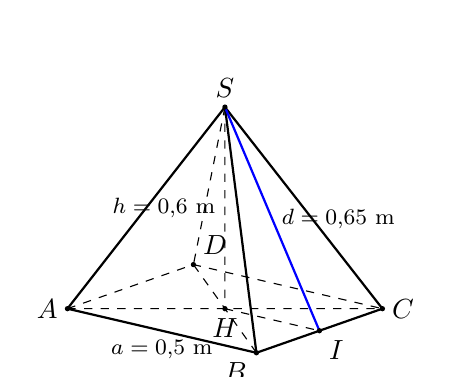
\begin{tikzpicture}[scale=0.8, >=stealth]
  \coordinate (A) at (0,0);
  \coordinate (B) at (3,-0.7);
  \coordinate (C) at (5,0);
  \coordinate (D) at (2,0.7);
  \coordinate (H) at ($(A)!0.5!(C)$);
  \coordinate (S) at ($(H)+(0,3.2)$);
  \coordinate (I) at ($(B)!0.5!(C)$);
  \draw[dashed] (A)--(D)--(C);
  \draw[dashed] (S)--(D);
  \draw[dashed] (A)--(C) (B)--(D);
  \draw[dashed] (S)--(H);
  \draw[dashed] (H)--(I);
  \draw[thick] (S)--(A)--(B)--(C)--(S);
  \draw[thick] (S)--(B);
  \draw[thick, blue] (S)--(I);
  \fill (A) circle (1.2pt) node[left] {$A$};
  \fill (B) circle (1.2pt) node[below left] {$B$};
  \fill (C) circle (1.2pt) node[right] {$C$};
  \fill (D) circle (1.2pt) node[above right] {$D$};
  \fill (S) circle (1.2pt) node[above] {$S$};
  \fill (H) circle (1.2pt) node[below] {$H$};
  \fill (I) circle (1.2pt) node[below right] {$I$};
  \node[left] at ($(S)!0.5!(H)$) {\footnotesize $h = 0{,}6\text{ m}$};
  \node[below] at ($(A)!0.5!(B)$) {\footnotesize $a = 0{,}5\text{ m}$};
  \node[right] at ($(S)!0.5!(I)$) {\footnotesize $d = 0{,}65\text{ m}$};
\end{tikzpicture}
\end{center}
\begin{enumerate}[label=\textbf{\alph*)}, leftmargin=0.8cm, itemsep=0pt, topsep=1pt]
\item (0,4 điểm) Tính thể tích khối bê tông.
\item (0,35 điểm) Người ta muốn sơn bốn mặt xung quanh của khối bê tông này. Biết chiều cao trung đoạn của hình chóp là $d = 0{,}65\text{ m}$. Tính diện tích bề mặt cần sơn.
\end{enumerate}
\loigiai{
\textbf{a)} \textit (0,4 điểm): Diện tích đáy hình vuông của khối bê tông là: $S_{\text{đáy}} = a^2 = 0{,}5 \cdot 0{,}5 = 0{,}25\text{ m}^2$.

Thể tích của khối bê tông là: $V = \dfrac{1}{3} S_{\text{đáy}} \cdot h = \dfrac{1}{3} \cdot 0{,}25 \cdot 0{,}6 = 0{,}05\text{ m}^3$.

\textbf{b)} \textit (0,35 điểm): Diện tích cần sơn chính là diện tích xung quanh của hình chóp tứ giác đều:

$S_{xq} = 4 \cdot \left(\dfrac{1}{2} a \cdot d\right) = 2 \cdot a \cdot d = 2 \cdot 0{,}5 \cdot 0{,}65 = 0{,}65\text{ m}^2$.


}
\end{ex}
\vspace{0.5mm}

\begin{ex} (0,5 điểm)
Tìm giá trị nhỏ nhất của biểu thức: $A = x^2 - 4x + y^2 + 6y + 15$.
\begin{enumerate}[label=\textbf{\alph*)}, leftmargin=0.8cm, itemsep=0pt, topsep=1pt]
\item (0,5 điểm) Tìm giá trị nhỏ nhất của $A$.
\end{enumerate}
\loigiai{
\textbf{a)} \textit (0,5 điểm): Biến đổi biểu thức $A$:

$A = (x^2 - 4x + 4) + (y^2 + 6y + 9) + 2 = (x - 2)^2 + (y + 3)^2 + 2$.

Vì $(x - 2)^2 \ge 0$ và $(y + 3)^2 \ge 0$ với mọi $x, y$, nên $A \ge 2$ với mọi $x, y$.

Dấu "=" xảy ra khi và chỉ khi: $\begin{cases} x - 2 = 0 \\ y + 3 = 0 \end{cases} \Leftrightarrow \begin{cases} x = 2 \\ y = -3 \end{cases}$.

Vậy giá trị nhỏ nhất của $A$ là $2$, đạt được khi $x = 2$ và $y = -3$.


}
\end{ex}
\vspace{0.5mm}


\enlargethispage{1.5cm}
\begin{center}
\rule{4cm}{0.4pt}\\
\textit{--- HẾT ---}
\end{center}
\end{document}
